\chapter{Benchmarking Python and Go application servers}

Traffic on Seznam.cz applications is high and it moves around a few thousands requests per second per one instance of an application. Python \cite{python} is used for most of our application servers, especially the Tornado framework \cite{tornado} which can handle requests asynchronously and is more lightweight \cite{flask-django-tornado} that frameworks like Django \cite{django} or Flask \cite{flask}. I~decided to benchmark such Python server and compare its performance with a server written in Go \cite{golang}. Go is a relatively young programming language, yet there are many big applications that use it. Kubernetes and Docker are both written in Go. There are also many libraries for Go, which makes it more interesting for us than Rust for example.

I~developed two simple servers which handle GET requests, generate HTML output based on a template and return the response. In Python I~used the Jinja2 \cite{jinja2} templating system, in Go I~relied on the built-in \lstinline{html/template} package. Both servers compose the output using a layout template and both render one variable in the template.

I~started those servers in Kubernetes and exposed their ports as a service. Then I~had to choose which benchmarking tool to use, so I~picked wrk \cite{wrk}.
 
Wrk is a modern HTTP benchmarking tool capable of generating a significant load when run on a single multi-core CPU. It combines a multithreaded design with scalable event notification systems such as epoll and kqueue \cite{wrk}.

Wrk allows to modify the number of client threads and the count connections opened simultaneously. I~started with 50 threads and 2000 connections opened at once. Each test was firstly start with 10 second interval for warming up the server and then repeated 3 times with 2 minute length.

I~started both servers in Kubernetes and allowed them to use only one CPU core. Then I~was adding cores to the servers and ran this test again and again.

For the testing I~used a bare-metal server with the Debian Jessie operating system installed. The hardware configuration of this machine was 24 Intel Xeon processors at 2.27 GHz and 32 GB of RAM. Both servers were running in Docker on one machine and I~used another one to run the benchmarks one after another.

The request rate per second is shown in the graph \ref{fig:benchmark-requests} and the average latency in the graph \ref{fig:benchmark-latency}.

From the graphs we can see that the Go application server is far much faster and is scaling linearly with the CPU count. The top boundary of the scaling was about 33 000 requests per second and was most likely held back by the network limits in the developer VLAN where my machines were placed. Python scales well in the beginning but with an increasing CPU count it starts to scale more slowly. Even with all of the 24 CPUs involved it didn’t achieved the performance of the Go server and that is a good reason to start writing our application servers in the Go language.

\begin{figure}[htb]\centering
  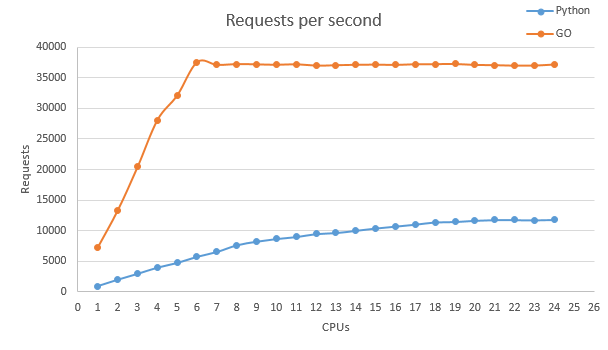
\includegraphics[width=1\textwidth]{images/benchmark-requests.png}
  \caption
    {Benchmarking Python and Go: Requests per second}
  \label{fig:benchmark-requests}
\end{figure}
                                                  
\begin{figure}[htb]\centering
  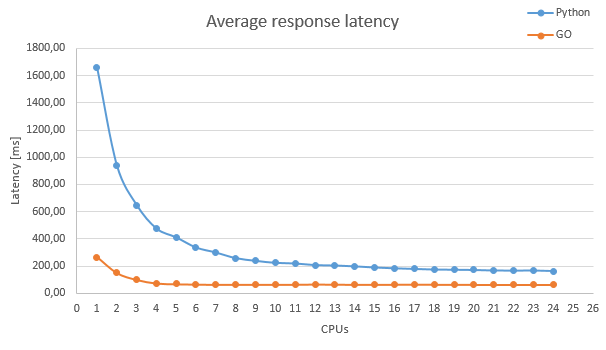
\includegraphics[width=1\textwidth]{images/benchmark-latency.png}
  \caption
    {Benchmarking Python and Go: Average response latency}
  \label{fig:benchmark-latency}
\end{figure}
                                                  
\begin{figure}[htb]\centering
  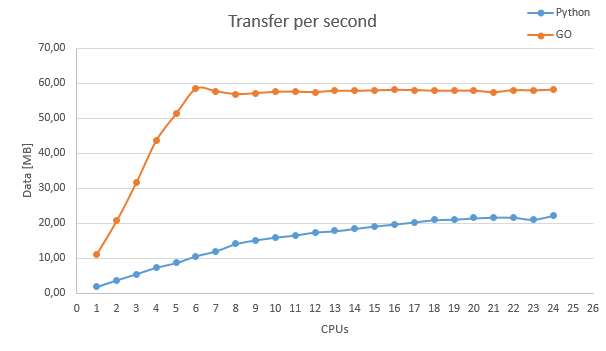
\includegraphics[width=1\textwidth]{images/benchmark-transfer.png}
  \caption
    {Benchmarking Python and Go: Transfer per second}
  \label{fig:benchmark-transfer}
\end{figure}